\chapter{Ең қысқа жолдар}

\index{ең қысқа жол}

Графтағы екі төбенің арасындағы ең қысқа жолды табу -- көптеген практикалық қолданысы бар маңызды есептердің бірі. Жол картасы мен барлық телімдердің ұзындығы белгілі болған жағдайда екі қала арасындағы төте маршрутты табу мәселесін оның айқын мысалы ретінде келтіруге болады.   
Салмақтанбаған графта жолдың ұзындығы жолдағы қырлардың
санына тең болады. Осындай жағдайда ең қысқа жолды табу үшін жай ғана ені бойынша ізденіс алгоритмін қолдансақ болады.
Алайда бұл тарауда біз салмақтанған графтарды қарастырамыз. 
Олармен жұмыс барысында қиынырақ алгоритмдерді
қолдануға мәжбүр боламыз.

\section{Беллман-Форд алгоритмі}

\index{Беллман-Форд алгоритмі}

\key{Беллман-Форд алгоритмі}\footnote{Алгоритм атауы американдық ғалымдар Ричард Беллман мен Лестер Фордтың құрметіне қойылған. Форд бұл алгоритмді 1956 жылы басқа математикалық есепті зерттеу кезінде ойлап тауып, жарияласа, Беллман 1958 жылы ең қысқа жолды табудың нақты міндеті туралы мақаласында береді \cite{bel58,for56a}.}бастапқы төбеден графтағы барлық
төбелерге дейін ең қысқа жолдарды табады.
Алгоритм графтың барлық түрлерімен жұмыс жасай алады. Бірақ
графта ұзындығы $0$-ден кем болатын цикл болмауы қажет.
Графта ұзындығы минус болатын цикл болса, алгоритм оны байқайды.

Алгоритм бастапқы төбеден графтың барлық төбелеріне
дейінгі қашықтықтарды қадағалайды. Алғашында
арақашықтықты бастапқы төбеден $0$-ге тең, ал басқалары үшін шексіздік
деп белгілейміз. Кейін алгоритм төбелер арасындағы арақашықтықты
мейлінше азайтатын қырларды іздейді. Егер де арақашықтықты қысқарту мүмкін
болмаса, алгоритм аяқталады.

\subsubsection{Мысал}

Келесі графта Беллман-Форд алгоритмі қалай жұмыс
жасайтынын қарастырамыз:
\begin{center}
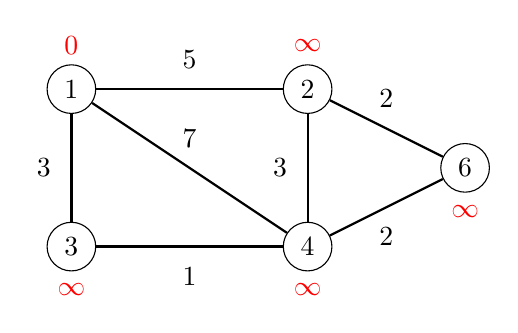
\begin{tikzpicture}
\node[draw, circle] (1) at (1,3) {1};
\node[draw, circle] (2) at (4,3) {2};
\node[draw, circle] (3) at (1,1) {3};
\node[draw, circle] (4) at (4,1) {4};
\node[draw, circle] (5) at (6,2) {6};
\node[color=red] at (1,3+0.55) {$0$};
\node[color=red] at (4,3+0.55) {$\infty$};
\node[color=red] at (1,1-0.55) {$\infty$};
\node[color=red] at (4,1-0.55) {$\infty$};
\node[color=red] at (6,2-0.55) {$\infty$};
\path[draw,thick,-] (1) -- node[font=\small,label=above:5] {} (2);
\path[draw,thick,-] (1) -- node[font=\small,label=left:3] {} (3);
\path[draw,thick,-] (3) -- node[font=\small,label=below:1] {} (4);
\path[draw,thick,-] (2) -- node[font=\small,label=left:3] {} (4);
\path[draw,thick,-] (2) -- node[font=\small,label=above:2] {} (5);
\path[draw,thick,-] (4) -- node[font=\small,label=below:2] {} (5);
\path[draw,thick,-] (1) -- node[font=\small,label=above:7] {} (4);
\end{tikzpicture}
\end{center}
Біріншіден, графтың әр төбесіне арақашықтық тағайындалады. Бастапқы төбеге дейінгі арақашықтық $0$-ге тең, ал қалған барлық төбелерге дейінгісі -- шексіз.

Алгоритм қашықтықты азайтатын қырларды іздейді.
1-төбенің барлық қырлары азайта алады:
\begin{center}
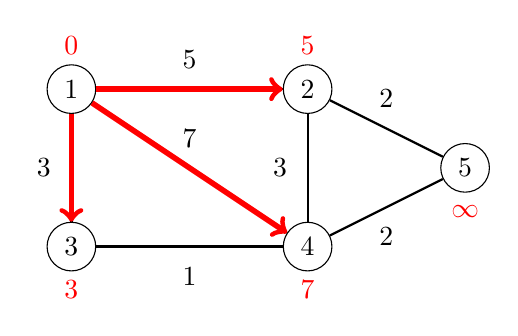
\begin{tikzpicture}
\node[draw, circle] (1) at (1,3) {1};
\node[draw, circle] (2) at (4,3) {2};
\node[draw, circle] (3) at (1,1) {3};
\node[draw, circle] (4) at (4,1) {4};
\node[draw, circle] (5) at (6,2) {5};
\node[color=red] at (1,3+0.55) {$0$};
\node[color=red] at (4,3+0.55) {$5$};
\node[color=red] at (1,1-0.55) {$3$};
\node[color=red] at (4,1-0.55) {$7$};
\node[color=red] at (6,2-0.55) {$\infty$};
\path[draw,thick,-] (1) -- node[font=\small,label=above:5] {} (2);
\path[draw,thick,-] (1) -- node[font=\small,label=left:3] {} (3);
\path[draw,thick,-] (3) -- node[font=\small,label=below:1] {} (4);
\path[draw,thick,-] (2) -- node[font=\small,label=left:3] {} (4);
\path[draw,thick,-] (2) -- node[font=\small,label=above:2] {} (5);
\path[draw,thick,-] (4) -- node[font=\small,label=below:2] {} (5);
\path[draw,thick,-] (1) -- node[font=\small,label=above:7] {} (4);

\path[draw=red,thick,->,line width=2pt] (1) -- (2);
\path[draw=red,thick,->,line width=2pt] (1) -- (3);
\path[draw=red,thick,->,line width=2pt] (1) -- (4);
\end{tikzpicture}
\end{center}
Содан кейін 
$2 \rightarrow 5$ және $3 \rightarrow 4$
қырлары қашықтықты қысқартады:
\begin{center}
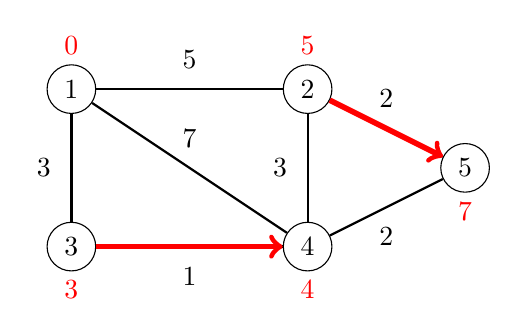
\begin{tikzpicture}
\node[draw, circle] (1) at (1,3) {1};
\node[draw, circle] (2) at (4,3) {2};
\node[draw, circle] (3) at (1,1) {3};
\node[draw, circle] (4) at (4,1) {4};
\node[draw, circle] (5) at (6,2) {5};
\node[color=red] at (1,3+0.55) {$0$};
\node[color=red] at (4,3+0.55) {$5$};
\node[color=red] at (1,1-0.55) {$3$};
\node[color=red] at (4,1-0.55) {$4$};
\node[color=red] at (6,2-0.55) {$7$};
\path[draw,thick,-] (1) -- node[font=\small,label=above:5] {} (2);
\path[draw,thick,-] (1) -- node[font=\small,label=left:3] {} (3);
\path[draw,thick,-] (3) -- node[font=\small,label=below:1] {} (4);
\path[draw,thick,-] (2) -- node[font=\small,label=left:3] {} (4);
\path[draw,thick,-] (2) -- node[font=\small,label=above:2] {} (5);
\path[draw,thick,-] (4) -- node[font=\small,label=below:2] {} (5);
\path[draw,thick,-] (1) -- node[font=\small,label=above:7] {} (4);

\path[draw=red,thick,->,line width=2pt] (2) -- (5);
\path[draw=red,thick,->,line width=2pt] (3) -- (4);
\end{tikzpicture}
\end{center}
Төменде соңғы өзгеріс көрсетіледі:
\begin{center}
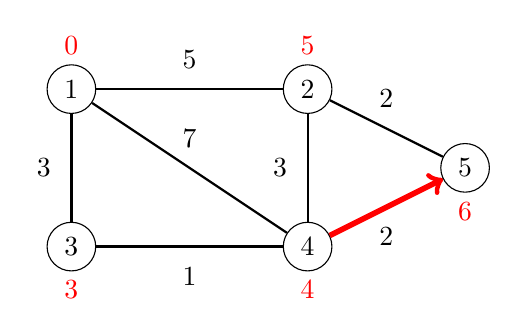
\begin{tikzpicture}
\node[draw, circle] (1) at (1,3) {1};
\node[draw, circle] (2) at (4,3) {2};
\node[draw, circle] (3) at (1,1) {3};
\node[draw, circle] (4) at (4,1) {4};
\node[draw, circle] (5) at (6,2) {5};
\node[color=red] at (1,3+0.55) {$0$};
\node[color=red] at (4,3+0.55) {$5$};
\node[color=red] at (1,1-0.55) {$3$};
\node[color=red] at (4,1-0.55) {$4$};
\node[color=red] at (6,2-0.55) {$6$};
\path[draw,thick,-] (1) -- node[font=\small,label=above:5] {} (2);
\path[draw,thick,-] (1) -- node[font=\small,label=left:3] {} (3);
\path[draw,thick,-] (3) -- node[font=\small,label=below:1] {} (4);
\path[draw,thick,-] (2) -- node[font=\small,label=left:3] {} (4);
\path[draw,thick,-] (2) -- node[font=\small,label=above:2] {} (5);
\path[draw,thick,-] (4) -- node[font=\small,label=below:2] {} (5);
\path[draw,thick,-] (1) -- node[font=\small,label=above:7] {} (4);

\path[draw=red,thick,->,line width=2pt] (4) -- (5);
\end{tikzpicture}
\end{center}

Осыдан кейін ешбір қыр арақашықтықты азайта алмайды.
Бұл арақашықтықтардың енді өзгермейтіндігін және біз
бастапқы төбеден басқа төбелерге дейінгі арақашықтықтарды 
есептеп шыққанымызды білдіреді.

Мысалы, $1$-төбеден $5$-төбеге дейінгі 
арақашықтығы $6$-ға тең ең қысқа жол осылай белгіленген:

\begin{center}
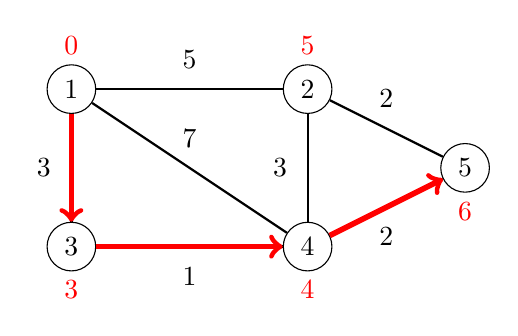
\begin{tikzpicture}
\node[draw, circle] (1) at (1,3) {1};
\node[draw, circle] (2) at (4,3) {2};
\node[draw, circle] (3) at (1,1) {3};
\node[draw, circle] (4) at (4,1) {4};
\node[draw, circle] (5) at (6,2) {5};
\node[color=red] at (1,3+0.55) {$0$};
\node[color=red] at (4,3+0.55) {$5$};
\node[color=red] at (1,1-0.55) {$3$};
\node[color=red] at (4,1-0.55) {$4$};
\node[color=red] at (6,2-0.55) {$6$};
\path[draw,thick,-] (1) -- node[font=\small,label=above:5] {} (2);
\path[draw,thick,-] (1) -- node[font=\small,label=left:3] {} (3);
\path[draw,thick,-] (3) -- node[font=\small,label=below:1] {} (4);
\path[draw,thick,-] (2) -- node[font=\small,label=left:3] {} (4);
\path[draw,thick,-] (2) -- node[font=\small,label=above:2] {} (5);
\path[draw,thick,-] (4) -- node[font=\small,label=below:2] {} (5);
\path[draw,thick,-] (1) -- node[font=\small,label=above:7] {} (4);

\path[draw=red,thick,->,line width=2pt] (1) -- (3);
\path[draw=red,thick,->,line width=2pt] (3) -- (4);
\path[draw=red,thick,->,line width=2pt] (4) -- (5);
\end{tikzpicture}
\end{center}

\subsubsection{Кодтың жазылуы}

Төменде берілген Беллман-Форд алгоритмінің коды $x$ 
төбесінен графтың барлық төбелеріне дейінгі ең қысқа
арақашықтықты анықтайды. Кодта $(a,b,w)$
құрылымында сақталған \texttt{edges} қырлар
тізбегі қолданылады, яғни $a$ төбесінен $b$ төбесіне
дейін салмағы $w$-ге тең қыр бар.

Алгоритм қадамдарды $n-1$ рет қайталайды.
Әр қадамда графтағы барлық төбелерді
өтіп шығып, арақашықтықты азайтуға тырысады.
\texttt{distance} жиымы $x$ төбесінен 
барлық төбелерге дейінгі қашықтықты сақтайды.
Ал \texttt{INF} тұрақтыcы шексіздікті
білдіреді.
\begin{lstlisting}
for (int i = 1; i <= n; i++) distance[i] = INF;
distance[x] = 0;
for (int i = 1; i <= n-1; i++) {
    for (auto e : edges) {
        int a, b, w;
        tie(a, b, w) = e;
        distance[b] = min(distance[b], distance[a]+w);
    }
}
\end{lstlisting}

Алгоритмнің уақытша күрделілігі -- $O(nm)$. 
Себебі алгоритм $n-1$ қадам жасайды және әр қадамда 
графтағы барлық $m$ қырды өтіп шығады.
Егер де графта ұзындығы минус цикл болмаса,
$n-1$ қадамнан кейін графтағы барлық арақашықтық
ең тиімді болады. Себебі, әр ең қысқа жол $n-1$ 
санынан көп қыр қамти алмайды.

Түпкілікті арақашықтық әдетте барлық $n-1$ айналым жасалмастан бұрын-ақ белгілі болады. Сол себепті кезекті айналымда ешбір арақашықтық азаймаса, алгоритмді жай ғана тоқтата салуға болады.

\subsubsection{Теріс цикл}

\index{теріс цикл}

Беллман-Форд алгоритмі арқылы графта теріс 
цикл (ұзындығы $0$-ден кем болатын цикл) бар-жоғын тексеруге болады.
Мысалға төмендегі графты алайық:

\begin{center}
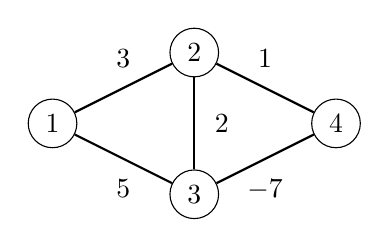
\begin{tikzpicture}[scale=0.9]
\node[draw, circle] (1) at (0,0) {$1$};
\node[draw, circle] (2) at (2,1) {$2$};
\node[draw, circle] (3) at (2,-1) {$3$};
\node[draw, circle] (4) at (4,0) {$4$};

\path[draw,thick,-] (1) -- node[font=\small,label=above:$3$] {} (2);
\path[draw,thick,-] (2) -- node[font=\small,label=above:$1$] {} (4);
\path[draw,thick,-] (1) -- node[font=\small,label=below:$5$] {} (3);
\path[draw,thick,-] (3) -- node[font=\small,label=below:$-7$] {} (4);
\path[draw,thick,-] (2) -- node[font=\small,label=right:$2$] {} (3);
\end{tikzpicture}
\end{center}
\noindent
Бұл графта $2 \rightarrow 3 \rightarrow 4 \rightarrow 2$ ұзындығы -4 болатын теріс цикл бар.
 
Бұл жағдайда мұндай циклды қамтитын кез келген жолдың ұзындығын шексіз азайтуға болады, сондықтан ең қысқа жол ұғымы мағынасын жоғалтады.

Графта теріс цикл бар-жоғын Беллман-Форд
алгоритмін $n$ қадамға созу арқылы тексеруге
болады. Біз графтағы барлық төбелерге ең қысқа жолды табу үшін 
$n-1$ қадам жеткілікті екенін білеміз. Бірақ граф теріс 
циклды камтыса, алгоритм $n$ қадамда да басқа қысқа 
жолды табады. Осылайша тағы бір қадам жасап, графты теріс циклға
тексеруге болады. Бұл алгоритмнің бастапқы төбенің таңдалуына қарамастан, теріс циклды көрсететінін атап өтпекпіз. 

\subsubsection{SPFA алгоритмі}

\index{SPFA алгорим}

\key{SPFA алгоритмі} (''Shortest Path Faster Algorithm'') \cite{fan94} --
Беллман-Форд алгоритмінің жылдамырақ нұсқасы.
SPFA алгоритмі графтағы барлық қырларды өтпейді. Ол қарастырылатын қырларды ақылды түрде өтіп шығады.

Алгоритм арақашықтықтарды қысқарту үшін пайдаланылуы
мүмкін төбелердің кезегін сақтайды.
Алдымен кезекке бастапқы $x$ төбесін
енгізеді.
Кейін кезектегі бірінші төбені алып, 
сол төбеден шығатын қырларды қарастырады. Егер 
$a \rightarrow b$ қыры арақашықтықты азайтса, $b$
төбесі кезекке қосылады.
%
% The following implementation uses a 
% \texttt{queue} \texttt{q}.
% In addition, an array \texttt{inqueue} indicates
% if a node is already in the queue,
% in which case the algorithm does not add
% the node to the queue again.

% \begin{lstlisting}
% for (int i = 1; i <= n; i++) distance[i] = INF;
% distance[x] = 0;
% q.push(x);
% while (!q.empty()) {
%     int a = q.front(); q.pop();
%     inqueue[a] = false;
%     for (auto b : v[a]) {
%         if (distance[a]+b.second < distance[b.first]) {
%             distance[b.first] = distance[a]+b.second;
%             if (!inqueue[b]) {q.push(b); inqueue[b] = true;}
%         }
%     }
% }
% \end{lstlisting}
%

SPFA алгоритмінің тиімділігі графтың құрылымына тікелей 
байланысты: алгоритм көбіне тиімді, бірақ оның уақытша күрделілігі ең нашар дегенде $O(nm)$ болады және алгоритмді Беллман-Форд алгоритмі сияқты баяу ететін кіріс деректерін құра аламыз.

\section{Дейкстра алгоритмі}

\index{Дейкстра алгоритмі}

\key{Дейкстра алгоритмі}\footnote{Бұл алгоритмді 1959 жылы Е.В.Дейкстра жариялаған еді \cite{dij59};
Дегенмен түпнұсқа еңбекте алгоритмді тиімді жүзеге асыру жолы жазылмаған болатын.}
де Беллман-Форд алгоритмі сияқты бастапқы төбеден графтың барлық
төбелеріне дейінгі ең қысқа жолдарды табады.
Дейкстра алгоритмінің артықшылығы -- оның тиімділігінде және
үлкен графтармен жұмыс жасай алуында.
Дегенмен алгоритм жұмыс жасау үшін граф ішінде 
салмағы теріс болатын қыр болмауы керек.

Беллман-Форд алгоритмі сияқты Дейкстра алгоритмі
төбелерге дейінгі арақашықтықты сақтайды және  
іздеу кезінде оларды біртіндеп азайтады.
Графта теріс салмақты қыр болмағандықтан, Дейкстра алгоритмі әр қырмен
тек бір рет жұмыс жасайды және осыған байланысты жылдам болып келеді.

\subsubsection{Мысал}

Келесі графта бастапқы төбесі $1$ болатын Дейкстра алгоритмінің қалай жұмыс 
істейтінін қарастырамыз:
\begin{center}
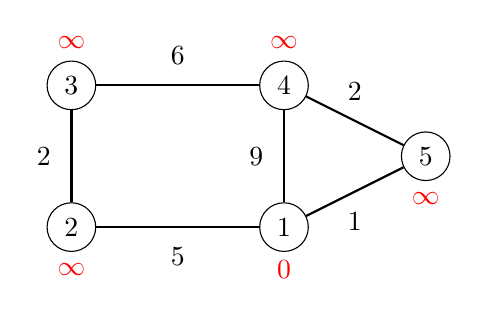
\begin{tikzpicture}[scale=0.9]
\node[draw, circle] (1) at (1,3) {3};
\node[draw, circle] (2) at (4,3) {4};
\node[draw, circle] (3) at (1,1) {2};
\node[draw, circle] (4) at (4,1) {1};
\node[draw, circle] (5) at (6,2) {5};

\node[color=red] at (1,3+0.6) {$\infty$};
\node[color=red] at (4,3+0.6) {$\infty$};
\node[color=red] at (1,1-0.6) {$\infty$};
\node[color=red] at (4,1-0.6) {$0$};
\node[color=red] at (6,2-0.6) {$\infty$};

\path[draw,thick,-] (1) -- node[font=\small,label=above:6] {} (2);
\path[draw,thick,-] (1) -- node[font=\small,label=left:2] {} (3);
\path[draw,thick,-] (3) -- node[font=\small,label=below:5] {} (4);
\path[draw,thick,-] (2) -- node[font=\small,label=left:9] {} (4);
\path[draw,thick,-] (2) -- node[font=\small,label=above:2] {} (5);
\path[draw,thick,-] (4) -- node[font=\small,label=below:1] {} (5);
\end{tikzpicture}
\end{center}
Беллман-Форд алгоритміндегідей қашықтық бастапқы төбе үшін  
$0$-ге, ал қалған төбелер үшін шексіздікке тең.

Әр қадам сайын Дейкстра алгоритмі қолданылмаған
және қашықтығы ең аз төбені таңдайды. Ең алғашқы қарастырылатын төбе --
қашықтығы $0$-ге тең $1$-төбе.

Төбе таңдалғанда, алгоритм содан шығып тұрған 
барлық қырларды өтіп шығып, басқа төбелерге қашықтықты 
азайтуын тексереді:
\begin{center}
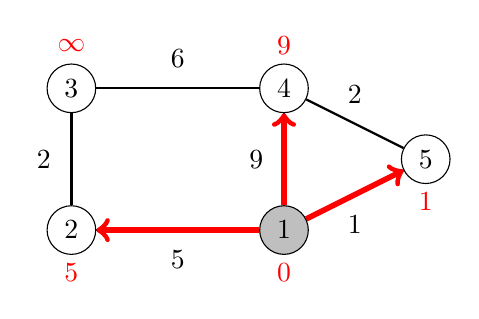
\begin{tikzpicture}[scale=0.9]
\node[draw, circle] (1) at (1,3) {3};
\node[draw, circle] (2) at (4,3) {4};
\node[draw, circle] (3) at (1,1) {2};
\node[draw, circle, fill=lightgray] (4) at (4,1) {1};
\node[draw, circle] (5) at (6,2) {5};

\node[color=red] at (1,3+0.6) {$\infty$};
\node[color=red] at (4,3+0.6) {$9$};
\node[color=red] at (1,1-0.6) {$5$};
\node[color=red] at (4,1-0.6) {$0$};
\node[color=red] at (6,2-0.6) {$1$};

\path[draw,thick,-] (1) -- node[font=\small,label=above:6] {} (2);
\path[draw,thick,-] (1) -- node[font=\small,label=left:2] {} (3);
\path[draw,thick,-] (3) -- node[font=\small,label=below:5] {} (4);
\path[draw,thick,-] (2) -- node[font=\small,label=left:9] {} (4);
\path[draw,thick,-] (2) -- node[font=\small,label=above:2] {} (5);
\path[draw,thick,-] (4) -- node[font=\small,label=below:1] {} (5);

\path[draw=red,thick,->,line width=2pt] (4) -- (2);
\path[draw=red,thick,->,line width=2pt] (4) -- (3);
\path[draw=red,thick,->,line width=2pt] (4) -- (5);
\end{tikzpicture}
\end{center}
Осы жағдайда $1$-төбеден шығып тұрған қырлар 
$2$, $4$ және $5$ төбелеріне арақашықтықты қысқартты. Олардың
арақашықтығы енді сәйкесінше 5, 9 және 1.

Келесі қарастырылатын төбе арақашықтығы $1$-ге тең $5$-төбе.
Ол $4$-төбенің арақашықтығын $9$-дан $3$-ке азайтты:
\begin{center}
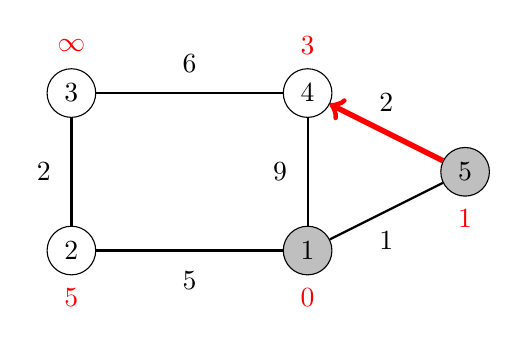
\begin{tikzpicture}
\node[draw, circle] (1) at (1,3) {3};
\node[draw, circle] (2) at (4,3) {4};
\node[draw, circle] (3) at (1,1) {2};
\node[draw, circle, fill=lightgray] (4) at (4,1) {1};
\node[draw, circle, fill=lightgray] (5) at (6,2) {5};

\node[color=red] at (1,3+0.6) {$\infty$};
\node[color=red] at (4,3+0.6) {$3$};
\node[color=red] at (1,1-0.6) {$5$};
\node[color=red] at (4,1-0.6) {$0$};
\node[color=red] at (6,2-0.6) {$1$};

\path[draw,thick,-] (1) -- node[font=\small,label=above:6] {} (2);
\path[draw,thick,-] (1) -- node[font=\small,label=left:2] {} (3);
\path[draw,thick,-] (3) -- node[font=\small,label=below:5] {} (4);
\path[draw,thick,-] (2) -- node[font=\small,label=left:9] {} (4);
\path[draw,thick,-] (2) -- node[font=\small,label=above:2] {} (5);
\path[draw,thick,-] (4) -- node[font=\small,label=below:1] {} (5);

\path[draw=red,thick,->,line width=2pt] (5) -- (2);
\end{tikzpicture}
\end{center}
Ендігі қарастырылатын төбе -- $4$-төбе. Ол $3$-төбеге дейінгі арақашықтықты $9$-ға төмендетті:
\begin{center}
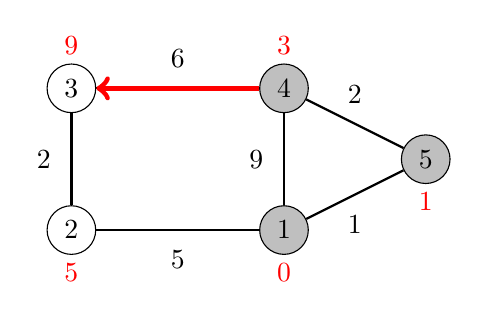
\begin{tikzpicture}[scale=0.9]
\node[draw, circle] (1) at (1,3) {3};
\node[draw, circle, fill=lightgray] (2) at (4,3) {4};
\node[draw, circle] (3) at (1,1) {2};
\node[draw, circle, fill=lightgray] (4) at (4,1) {1};
\node[draw, circle, fill=lightgray] (5) at (6,2) {5};

\node[color=red] at (1,3+0.6) {$9$};
\node[color=red] at (4,3+0.6) {$3$};
\node[color=red] at (1,1-0.6) {$5$};
\node[color=red] at (4,1-0.6) {$0$};
\node[color=red] at (6,2-0.6) {$1$};

\path[draw,thick,-] (1) -- node[font=\small,label=above:6] {} (2);
\path[draw,thick,-] (1) -- node[font=\small,label=left:2] {} (3);
\path[draw,thick,-] (3) -- node[font=\small,label=below:5] {} (4);
\path[draw,thick,-] (2) -- node[font=\small,label=left:9] {} (4);
\path[draw,thick,-] (2) -- node[font=\small,label=above:2] {} (5);
\path[draw,thick,-] (4) -- node[font=\small,label=below:1] {} (5);

\path[draw=red,thick,->,line width=2pt] (2) -- (1);
\end{tikzpicture}
\end{center}

Бір төбе таңдалғанда 
оның арақашықтығының түпкі  (яғни ең оңтайлы) болып табылуы Дейкстра алгоритмінің тамаша қасиетіне жатады.
Мысалы, қазіргі сәтте 0, 1 және 3 арақашықтықтары 1, 5 және 4
төбелеріне түпкі болып саналады.

Алгоритм қалған екі төбемен жұмыс жасайды, түпкі арақашықтықтар төмендегідей болмақ:

\begin{center}
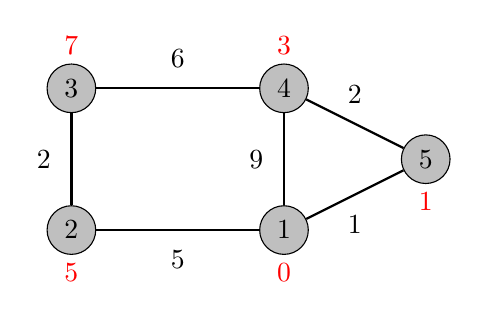
\begin{tikzpicture}[scale=0.9]
\node[draw, circle, fill=lightgray] (1) at (1,3) {3};
\node[draw, circle, fill=lightgray] (2) at (4,3) {4};
\node[draw, circle, fill=lightgray] (3) at (1,1) {2};
\node[draw, circle, fill=lightgray] (4) at (4,1) {1};
\node[draw, circle, fill=lightgray] (5) at (6,2) {5};

\node[color=red] at (1,3+0.6) {$7$};
\node[color=red] at (4,3+0.6) {$3$};
\node[color=red] at (1,1-0.6) {$5$};
\node[color=red] at (4,1-0.6) {$0$};
\node[color=red] at (6,2-0.6) {$1$};

\path[draw,thick,-] (1) -- node[font=\small,label=above:6] {} (2);
\path[draw,thick,-] (1) -- node[font=\small,label=left:2] {} (3);
\path[draw,thick,-] (3) -- node[font=\small,label=below:5] {} (4);
\path[draw,thick,-] (2) -- node[font=\small,label=left:9] {} (4);
\path[draw,thick,-] (2) -- node[font=\small,label=above:2] {} (5);
\path[draw,thick,-] (4) -- node[font=\small,label=below:1] {} (5);
\end{tikzpicture}
\end{center}

\subsubsection{Теріс қырлар}

Дейкстра алгоритмінің тиімділігі графта теріс қыр 
жоқтығына негізделген.
Егер теріс қыр болса алгоритм қате жауап беруі
мүмкін.
Мысалға, келесі графты қарастырайық:

\begin{center}
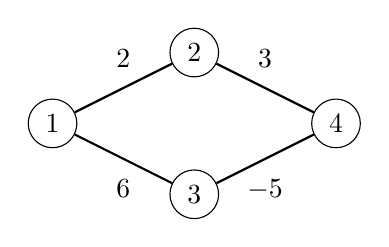
\begin{tikzpicture}[scale=0.9]
\node[draw, circle] (1) at (0,0) {$1$};
\node[draw, circle] (2) at (2,1) {$2$};
\node[draw, circle] (3) at (2,-1) {$3$};
\node[draw, circle] (4) at (4,0) {$4$};

\path[draw,thick,-] (1) -- node[font=\small,label=above:2] {} (2);
\path[draw,thick,-] (2) -- node[font=\small,label=above:3] {} (4);
\path[draw,thick,-] (1) -- node[font=\small,label=below:6] {} (3);
\path[draw,thick,-] (3) -- node[font=\small,label=below:$-5$] {} (4);
\end{tikzpicture}
\end{center}
\noindent
$1$-төбеден $4$-төбеге дейінгі ең қысқа жол $1 \rightarrow 3 \rightarrow 4$-ке, ал оның ұзындығы 1-ге тең.
Бірақ Дейкстра алгоритмі ең аз салмақтағы қырларға ілесе отырып, $1 \rightarrow 2 \rightarrow 4$ деген жолды табады.
Алгоритм басқа жолда $-5$-ке тең салмақ алдыңғы $6$-ға тең үлкен  салмақтың орнын толтыратынын ескермейді.

\subsubsection{Кодтың жазылуы}

Жазылған келесі код бастапқы $x$ төбесінен графтағы
басқа төбелерге дейінгі ең қысқа арақашықты есептейді.
Графтың қырлары cыбайластық тізімі арқылы сақталған. 
Егер $a$ төбесінен $b$ төбесіне салмағы $w$ болатын қыр болса,
\texttt{adj[$a$]} векторы $(b,w)$ жұбын
сақтайды.

Дейкстра алгоритмінің тиімді үлгісі қолданылмаған
ең аз қашықтықтағы төбені табудың тиімді жолдарын талап етеді.
Осы ретте, төбелерді арақашықтығы бойынша
реттейтін басымдылық кезегі жарамды деректер құрылымы
саналады.
Басымдылық кезегі арқылы келесі қарастырылатын төбені
табу үшін логаримфдік уақыт жұмсалады.

Берілген кодта басымдылық кезегі $(-d,x)$ жұптарын сақтайды.
Жұп қазіргі уақытта $x$-төбеге дейінгі қашықтық $d$ екенін көрсетеді.
$\texttt{distance}$ жиымы әрбір төбеге дейінгі қашықтықты қамтиды және
$\texttt{processed}$ жиымы төбенің өңделгенін немесе
өңделмегенін көрсетеді.
Басында $x$-төбенің арақашықтығы $0$-ге, ал басқа төбелер үшін $\infty$ тең.

\begin{lstlisting}
for (int i = 1; i <= n; i++) distance[i] = INF;
distance[x] = 0;
q.push({0,x});
while (!q.empty()) {
    int a = q.top().second; q.pop();
    if (processed[a]) continue;
    processed[a] = true;
    for (auto u : adj[a]) {
        int b = u.first, w = u.second;
        if (distance[a]+w < distance[b]) {
            distance[b] = distance[a]+w;
            q.push({-distance[b],b});
        }
    }
}
\end{lstlisting}

Басымдылық кезегінде арақашықтықты минус белгісімен
сақтайтынымызды ескеруіміз керек. C++ ішіндегі 
басымдылық кезегі максималды элементтерді табатындықтан, ал бізге минималды элементтер қажет болғандықтан біз осылай сақтауға мәжбүрміз.
Минус белгісін қою арқылы біз тікелей әдепкі басымдылық
кезегімен жұмыс жасай аламыз\footnote{Әрине кезекті 4.5 тарауында сипатталғандай етіп жариялауға және оң қашықтықтарды пайдалануға болар еді, алайда бұл кезде код ұзақ болып кетеді.}.

Басымдылық кезегінде бір төбенің бірнеше данасы
болуы мүмкін екендігін де ескеріңіз. Дегенмен ең аз қашықтықтағы данасы ғана өңделеді.

Жоғарыдағы кодтың уақытша күрделілігі -- $O(n+m \log m)$.
Себебі алгоритм графтағы барлық төбелерді өтіп шығады және 
әр қырдан көп дегенде бір арақашықтықты басымдылық кезегіне қосады.

\section{Флойд-Уоршелл алгоритмі}

\index{Флойд-Уоршелл алгоритмі}

\key{Флойд-Уоршелл алгоритмі}\footnote{Алгоритм 1962 жылы оны дербес жариялаған Р.В.Флойд пен С.Уоршеллдің құрметіне аталған. \cite{flo62,war62}.}
ең қысқа жолдарды табу есебіне басқаша тәсіл ұсынады.
Басқа алгоритмдерге қарағанда, ол төбелер арасындағы барлық қысқа жолдарды бір өту арқылы табатындығымен ерекшеленеді.

Алгоритм төбелер жұбының арақашықтығынан тұратын матрицаны қолдайды. Бастапқы сәтте матрица сыбайлас матрица негізінде меншіктейді.   
Содан кейін алгоритм бірнеше айналымдарды орындап, әр айналымда алдағы уақытта жолдың аралық төбесі болуы мүмкін жаңа төбені таңдайды.  Сол төбені пайдалана отырып, қашықтықты азайтады.

\subsubsection{Мысал}

Төмендегі графта Флойд-Уоршелл алгоритмі  
қалай жұмыс істейтінін қарастырамыз:

\begin{center}
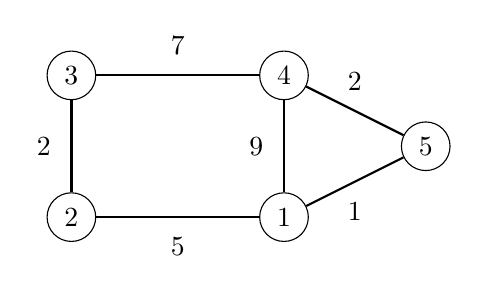
\begin{tikzpicture}[scale=0.9]
\node[draw, circle] (1) at (1,3) {$3$};
\node[draw, circle] (2) at (4,3) {$4$};
\node[draw, circle] (3) at (1,1) {$2$};
\node[draw, circle] (4) at (4,1) {$1$};
\node[draw, circle] (5) at (6,2) {$5$};

\path[draw,thick,-] (1) -- node[font=\small,label=above:7] {} (2);
\path[draw,thick,-] (1) -- node[font=\small,label=left:2] {} (3);
\path[draw,thick,-] (3) -- node[font=\small,label=below:5] {} (4);
\path[draw,thick,-] (2) -- node[font=\small,label=left:9] {} (4);
\path[draw,thick,-] (2) -- node[font=\small,label=above:2] {} (5);
\path[draw,thick,-] (4) -- node[font=\small,label=below:1] {} (5);
\end{tikzpicture}
\end{center}

Алғашында әр төбеден өзіне дейінгі арақашықтық $0$-ге,
ал егер $a$ мен $b$ төбелерінің арасында салмағы $x$ 
болатын қыр болса, арақашықтық $x$-ке тең болады.
Қалған арақашықтарды шексіздікке теңейміз.

Бұл граф үшін бастапқы жиым:
\begin{center}
\begin{tabular}{r|rrrrr}
 & 1 & 2 & 3 & 4 & 5 \\
\hline
1 & 0 & 5 & $\infty$ & 9 & 1 \\
2 & 5 & 0 & 2 & $\infty$ & $\infty$ \\
3 & $\infty$ & 2 & 0 & 7 & $\infty$ \\
4 & 9 & $\infty$ & 7 & 0 & 2 \\
5 & 1 & $\infty$ & $\infty$ & 2 & 0 \\
\end{tabular}
\end{center}
\vspace{10pt}

Алгоритм бірнеше дәйекті айналымдардан тұрады.
Әр айналымда алгоритм бір төбені таңдап, төбелер
арасындағы арақашықтықтарды таңдалған төбе арқылы
азайтуға тырысады.

Алғашқы айналымда $1$-төбе аралық төбе болады. $1$-төбе оларды байланыстырып тұрғандықтан, $2$ және $4$-төбелер арасындағы арақашықтығы $14$-ке,
ал $2$ мен $5$-төбелер арасында $6$-ға жаңарады.

\begin{center}
\begin{tabular}{r|rrrrr}
 & 1 & 2 & 3 & 4 & 5 \\
\hline
1 & 0 & 5 & $\infty$ & 9 & 1 \\
2 & 5 & 0 & 2 & \textbf{14} & \textbf{6} \\
3 & $\infty$ & 2 & 0 & 7 & $\infty$ \\
4 & 9 & \textbf{14} & 7 & 0 & 2 \\
5 & 1 & \textbf{6} & $\infty$ & 2 & 0 \\
\end{tabular}
\end{center}
\vspace{10pt}

Екінші айналымда $2$-төбе таңдалады.
$1$ мен $3$-төбелер және $3$ мен $5$-төбелер арасында арақашықтық жаңарады.

\begin{center}
\begin{tabular}{r|rrrrr}
 & 1 & 2 & 3 & 4 & 5 \\
\hline
1 & 0 & 5 & \textbf{7} & 9 & 1 \\
2 & 5 & 0 & 2 & 14 & 6 \\
3 & \textbf{7} & 2 & 0 & 7 & \textbf{8} \\
4 & 9 & 14 & 7 & 0 & 2 \\
5 & 1 & 6 & \textbf{8} & 2 & 0 \\
\end{tabular}
\end{center}
\vspace{10pt}

Үшінші айналымда, $3$-төбе таңдалынады.
Осы төбе $2$ мен $4$ арасында арақашықтықты азайтады.

\begin{center}
\begin{tabular}{r|rrrrr}
 & 1 & 2 & 3 & 4 & 5 \\
\hline
1 & 0 & 5 & 7 & 9 & 1 \\
2 & 5 & 0 & 2 & \textbf{9} & 6 \\
3 & 7 & 2 & 0 & 7 & 8 \\
4 & 9 & \textbf{9} & 7 & 0 & 2 \\
5 & 1 & 6 & 8 & 2 & 0 \\
\end{tabular}
\end{center}
\vspace{10pt}

Алгоритм барлық төбелерді қарап шыққанға дейін
осылай жалғаса береді. Соңында жиым екі төбелер
арасындағы минималды арақашықтарды қамтиды.

\begin{center}
\begin{tabular}{r|rrrrr}
 & 1 & 2 & 3 & 4 & 5 \\
\hline
1 & 0 & 5 & 7 & 3 & 1 \\
2 & 5 & 0 & 2 & 8 & 6 \\
3 & 7 & 2 & 0 & 7 & 8 \\
4 & 3 & 8 & 7 & 0 & 2 \\
5 & 1 & 6 & 8 & 2 & 0 \\
\end{tabular}
\end{center}

Мысалы, осы жиым бізге $2$ мен $4$-төбелер
арасында ең қысқа жолдың арақашықтығы $8$ екенін
көрсетеді.
Ол келесі жолға сәйкес келеді:

\begin{center}
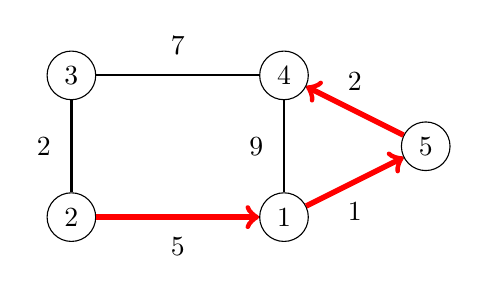
\begin{tikzpicture}[scale=0.9]
\node[draw, circle] (1) at (1,3) {$3$};
\node[draw, circle] (2) at (4,3) {$4$};
\node[draw, circle] (3) at (1,1) {$2$};
\node[draw, circle] (4) at (4,1) {$1$};
\node[draw, circle] (5) at (6,2) {$5$};

\path[draw,thick,-] (1) -- node[font=\small,label=above:7] {} (2);
\path[draw,thick,-] (1) -- node[font=\small,label=left:2] {} (3);
\path[draw,thick,-] (3) -- node[font=\small,label=below:5] {} (4);
\path[draw,thick,-] (2) -- node[font=\small,label=left:9] {} (4);
\path[draw,thick,-] (2) -- node[font=\small,label=above:2] {} (5);
\path[draw,thick,-] (4) -- node[font=\small,label=below:1] {} (5);

\path[draw=red,thick,->,line width=2pt] (3) -- (4);
\path[draw=red,thick,->,line width=2pt] (4) -- (5);
\path[draw=red,thick,->,line width=2pt] (5) -- (2);
\end{tikzpicture}
\end{center}

\subsubsection{Кодтың жазылуы}


Флойд-Уоршалл алгоритмінің артықшылығы - кодтың оңай жазылуында.
Келесі кодта $\texttt{distance}[a][b]$ $a$ мен $b$ арасындағы
ең қысқа жолды сақтайтын жиым жарияланған.
Алдымен \texttt{distance} жиымын \texttt{adj} cыбайластық матрицасы
арқылы меншіктейміз.

\begin{lstlisting}
for (int i = 1; i <= n; i++) {
    for (int j = 1; j <= n; j++) {
        if (i == j) distance[i][j] = 0;
        else if (adj[i][j]) distance[i][j] = adj[i][j];
        else distance[i][j] = INF;
    }
}
\end{lstlisting}
Содан кейін төмендегідей ретпен ең қысқа жолдарды табамыз: 
\begin{lstlisting}
for (int k = 1; k <= n; k++) {
    for (int i = 1; i <= n; i++) {
        for (int j = 1; j <= n; j++) {
            distance[i][j] = min(distance[i][j],
                                   distance[i][k]+distance[k][j]);
        }
    }
}
\end{lstlisting}

Аталған алгоритмнің уақытша күрделілігі $O(n^3)$. Себебі
алгоритм төбелерден өтетін үш кірістірілген 
циклді қамтиды.

Флойд-Уоршалл алгоритмін жүзеге асыру өте қарапайым 
болғандықтан, оны тіпті графтағы бір ғана қысқа жолды табу қажеттілігі туындаған жағдайда да ұсынуға болады. 
Алайда оны кубтық уақытша күрделілігі қолайлы жағдайда шағын графтар үшін ғана қолдана аламыз. 